\chapter{Analisi dei requisiti}
\section{Ideazione}
La maggior parte dei progetto richiede un breve passo iniziale in cui
si esaminano i seguenti tipi di domande:
\begin{itemize}
    \item Il progetto è fattibile?
    \item Comprare e/o costruire?
    \item Stima approssimativa e non affidabile dei costi
    \item Dovremmo procedere o fermarci?
\end{itemize}
L'ideazione non è la fase dei requisiti.
\\ Il problema principale che risolve l'ideazione è il seguente:
\begin{center}
    \textbf{Le parti interessate hanno un accordo di base, sulla visione
    del progetto, e vale la pena di investire un'indagine seria?}
\end{center}
Lo scopo è quindi quello di stabilire una visione comune per gli obiettivi del progetto
e capire se questo è fattibile.
\\ In questa fase non si utilizza molto UML (verrà utilizzato soprattutto durante
 l'elaborazione).
\paragraph*{Non hai capito l'ideazione se}
\begin{itemize}
    \item Dura più di qualche settimana
    \item Provi a definire molti requisiti
    \item Ci si aspetta che i piani e le stime siano affidabili
    \item I nomi di molti attori e casi d'uso non sono stati identificati
    \item Troppi casi d'uso sono stati scritti nel dettaglio
    \item Nessun caso d'uso è stato scritto in dettaglio
\end{itemize}
\section{Che sono sono i requisiti}
Un requisito è una capacità o una condizione a cui il sistema e più in generale il
progetto, deve essere conforme.
\\ I requisiti sono un aspetto veramente molto importante, si evidenzia
addirittura che 34 \% delle cause dei fallimenti dei progetti software
riguardano l'attività dei requisiti.
\paragraph*{Ci sono due tipi principali di requisiti}
\begin{itemize}
    \item Requisiti funzionali (comportamentali) - Descrivono il comportamento del
    sistema, in termini di funzionalità fornite ai suoi utenti e informazioni
    che il sistema deve gestire
    \item Requisiti non funzionali (tutti gli altri requisiti) - Sono relativi
    a proprietà del sistema nel suo complesso come per esempio sicurezza, presetazioni,
    scalabilità, usabilità...
\end{itemize}
\subsection{Requisiti funzionali}
Sono funzionalità o servizi che il sistema deve fornire, risposte che l'utente
aspetta dal software in determinate condizioni, risultati che il software deve produrre
in risposta a specifici input.
\paragraph{Il problema dell'imprecisione nella specifica dei requisiti}
Requisiti ambigui possono portare a diverse interpretazioni da sviluppatori e utenti.
In linea di principio i requisiti dovrebbero essere completi e coerenti, quindi
includere la definizione di tutti i servizi richiesti e non essere ambigui.
\subsection{Requisiti non funzionali}
Questi definiscono le proprietà e i vincoli del sistema, ad esempio affidabilità,
tempi di risposta, oppure vincoli come la capacità dei dispositivi I/O,
le rappresentazioni dei dati nelle interfacce di sistema, ecc.
\\I requisiti non funzionali possono essere più critici dei requisiti funzionali, dato che
in caso se non definiti correttamente il sistema potrebbe risultare inutilizzabile.
\paragraph*{Obiettivi e requisiti} I requisiti non funzionali possono essere molto
difficili da stabilire con precisione e requisiti imprecisi possono essere
difficili da verificare.
\\ Un obiettivo può essere un'intenzione generale dell'utente come la facilità d'uso,
mentre un requisito non funzionale verificabile è una dichiarazione che utilizza
alcune misure oggettivamente verificabili.
Gli obiettivi sono utili agli sviluppatori in quanto trasmettono le intenzioni degli
utenti del sistema.
\paragraph*{Metriche per specificare i requisiti non funzionali}
\begin{center}
    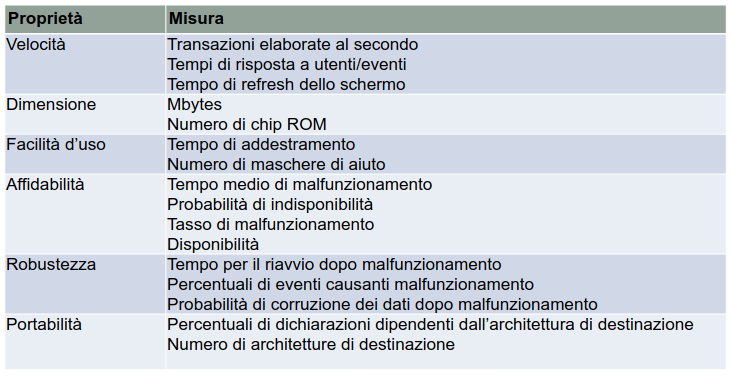
\includegraphics[width=100mm, scale=0.5]{metriche_requisiti_non_funzionali.png}
\end{center}
\subsection{Quali sono i modi validi per troavare requisiti}
\begin{itemize}
    \item Interviste con i clienti
    \item Scrivere casi d'uso con i clienti
    \item Workshop dei requisiti a cui partecipano sia sviluppatori che clienti
    \item Gruppi di lavoro con rappresentanti dei clienti
    \item Sollecitare feedback clienti alla fine di ogni iterazione
\end{itemize}
\section{Requisiti e principali elaborati di UP}
\begin{itemize}
    \item Modello dei casi d'uso
    \item Specifiche supplementari
    \item Glossario
    \item Visione
    \item Regole di Business
\end{itemize}
\paragraph*{Linee guida per la scrittura dei requisiti}
\begin{itemize}
    \item Ideare un formato standard e utilizzare per tutti i requisiti
    \item Utilizzo del linguaggio in modo consistente. Utilizzare DEVE per requisiti
    obbligatori, DOVREBBE per requisiti desiderabili
    \item Evidenziare porzioni di testo per identificare le parti più importanti dei requisiti
    \item Evitare gergo informatico
\end{itemize}

\chapter{Casi d'uso}
I casi d'uso sono storie scritte, ampiamente utilizzati per scoprire e registrare
i requisiti. Un caso d'uso è un dialogo tra un attore e un sistema che svolge un compito.
\\ I casi d'uso non sono elaborati orientati agli oggetti, influenzano però molti aspetti
di un progetto, compresa l'analisi e la progettazione orientata agli oggetti.
\textbf{I casi d'uso sono testo}.
\section{Attori, scenari e casi d'uso}
\begin{itemize}
    \item Un attore è qualcosa o qualcuno dotato di comportamento - Es. cassiere
    o sistema di pagamento 
    \item Uno scenario (o istanza del caso d'uso) è una sequenza specifica di azioni
    e iterazioni tra il sistema e alcuni attori - Descrive una particolare storia nell'uso
    del sistema, si possono dividere in scenari di successo e di fallimento.
    \item Un caso d'uso è una collezione di scenari correlati, sia di successo che
    di fallimento, che descrivono un attore che usa un sistema per raggiungere un
    obiettivo specifico
\end{itemize}
Il \textbf{Modello dei Casi d'Uso} è l'insieme di tutti i casi d'uso scritti.
\subsection{Perchè i casi d'uso}
Si tratta di un metodo semplice per descrivere i requisiti funzionali ed è
direttamente comprensibile dai clienti. Inoltre mettono in risalto obiettivi degli utenti
e il loro punto di vista. Molto utile per produrre la guida utente e per i test di sistema.
\paragraph*{I casi d'uso sono requisiti funzionali} Dato che essi indicano cosa
deve fare il sistema, un caso definisce un contratto relativo al comportamento
di un sistema.
\section{Tipi di Attore}
SuD = Sistema in discussione
\begin{itemize}
    \item Attore primario: raggiunge obiettivi usando il SuD
    \item Attore finale: vuole che il SuD sia utilizzato affinchè vengano raggiunti
    i suoi obiettivi (es cliente)
    \item Attore di supporto: es. servizio pagamento
    \item Attore fuori scena: ha un interessa nel comportamento del caso d'uso SuD, ma non
    è attore primario, finale o di supporto (es Governo interessanto al pagamento delle imposte)
\end{itemize}
\section{Tre formati comuni per i casi d'uso}
\begin{itemize}
    \item Formato breve - Riepilogo conciso di un solo paragrafo, normalmente relativo
    al solo scenario principale di successo
    \item Formato informale - Più paragrafi relativi anche agli altri scenari
    \item Formato dettagliato - Tutti i passi e le variazioni sono scritti nel dettaglio
\end{itemize}
\paragraph*{Formato Dettagliato}
\begin{center}
    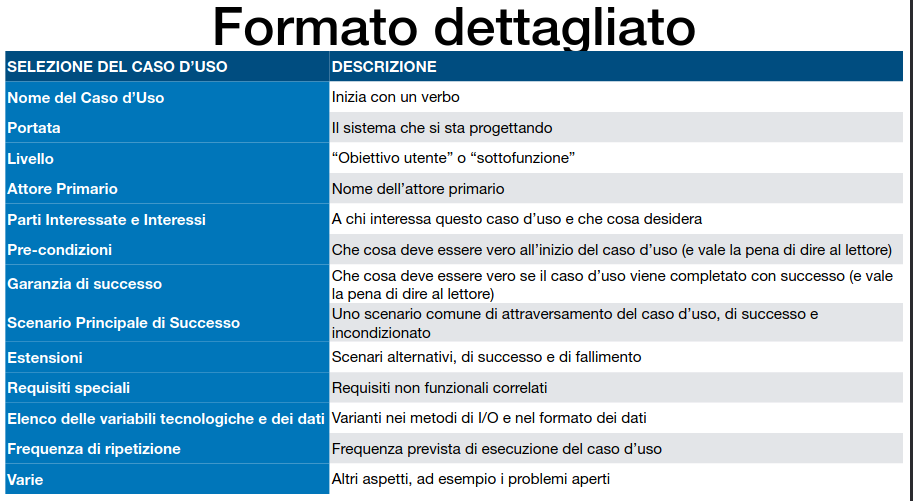
\includegraphics[width=100mm, scale=0.5]{caso_uso_format_dettaglio.png}
\end{center}
Scrivere in uno stile essenziale, come per esempio
\begin{itemize}
    \item L'amministratore si identifica
    \item Il sistema autentica l'identità
\end{itemize}
Scrivere casi d'uso in modo conciso e completo.
\\ Scrivere casi d'uso a scatola nera, ovvero speciricare che cosa
deve fare il sistema, senza decidere come lo farà.
Concentrarsi sulla comprensione di ciò che l'attore considera un risultato di valore.
\section{Come trovare i casi d'uso}
\begin{itemize}
    \item Scegliere il confine di sistema (Es identificando gli attori esterni)
    \item Identificare gli attori primari
    \item Identificare gli obiettivi per ogni attore primario
    \item Definire i casi d'uso che soddisfano questi obiettivi
\end{itemize}
Per dettagli leggere Capitolo 7 pag 88 del Larman 
\href{https://bookshelf.vitalsource.com/reader/books/9788891924193/pageid/116}{Link Bookshelf}.
\subsection{Verificare l'utilità dei casi d'uso}
Ci sono diversi metodi
\begin{itemize}
    \item Test del capo
    \item Test EBP (Elementary Business Process) - Capire se si tratta di un processo
    elementare e non troppo complesso
    \item Test della Dimensione - Un buon caso d'uso non dovrebbe essere troppo
    breve
\end{itemize}
\subsection{Livello dei casi d'uso}
I casi d'uso possono essere scritti a livelli diversi
\begin{itemize}
    \item Livello di obiettivo utente
    \item Livello di sotto-funzione
    \item Livello di sommario
\end{itemize}

\section{Diagramma dei Casi d'uso}
usare notazioni diverse per gli attori umani e per quelli che sono sistemi
informatici. Unire i vari attori e casi d'uso con associazioni rappresentate
da una linea continua. La direzione viene utilizzata nel verso di chi dà inizio
all'interazione.
\\ Non viene associata una direzione se entrambe le parti possono dare inizio
all'interazione.
\paragraph*{Relazioni tra Casi d'Uso}
\begin{itemize}
    \item Include - Relazione tra un caso d'uso base ed un caso d'uso incluso nel
    caso base
    \item Extend - Connette un caso d'uso esteso ad un caso d'uso base, aggiunge varianti
    ad un caso d'uso base e viene inserito solo se la condizione d'estensione è vera.
    \item Generalization - Un caso d'uso genitore è una generalizzazione di un caso d'uso
    figlio. Viene eseguito se la condizione di generalizzazione è vera. Possono ereditare, aggiungere
    sovrascrivere le funzioni del loro genitore. Si può avere anche tra attori questa
    relazione.
\end{itemize}
